\documentclass[12pt,a4paper]{report}
\RequirePackage[english,spanish,brazil,portuguese]{babel}
\RequirePackage[T1]{fontenc}
\RequirePackage{graphicx}
\graphicspath{{./logotipos/}{./figuras/}}
\PassOptionsToPackage{table}{xcolor}
\RequirePackage{pdfpages}
\RequirePackage{xspace}
\RequirePackage{setspace}
\RequirePackage{geometry}
\geometry{a4paper,top=30mm,bottom=20mm,left=30mm,right=20mm}
\RequirePackage[utf8]{inputenc}
\usepackage{indentfirst}
\usepackage{multirow}
\usepackage{float}
\usepackage{longtable} 

\begin{document}
\appendix
\chapter{}
\subsubsection{GCC}

\begin{figure}[H]
\centering

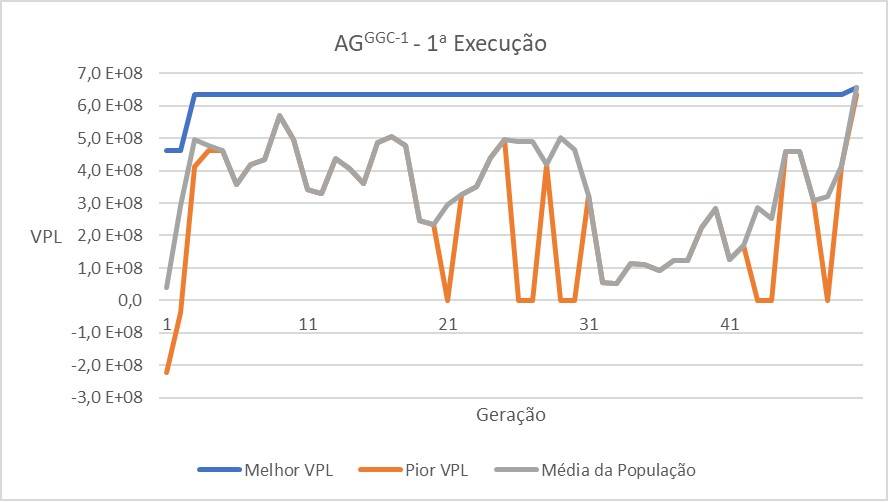
\includegraphics[scale=1]{ApA/GCC/1}
\end{figure}

\begin{figure}[H]
\centering

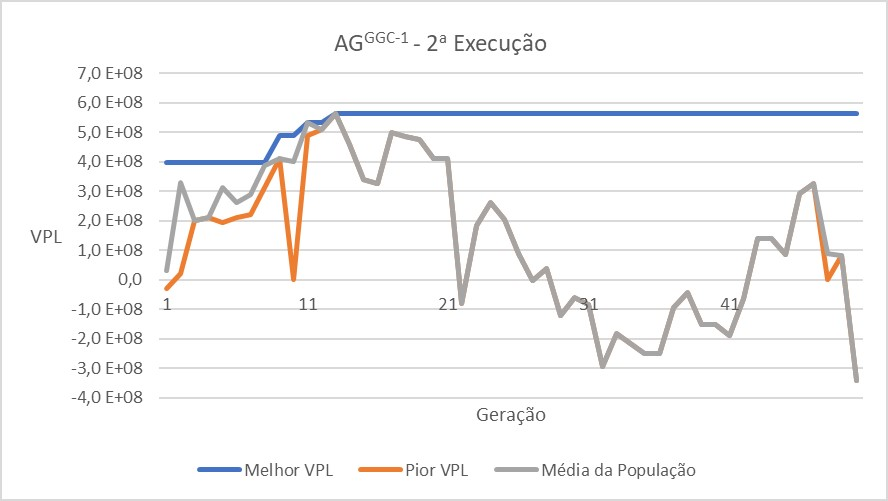
\includegraphics[scale=1]{ApA/GCC/2}
\end{figure}

\begin{figure}[H]
\centering

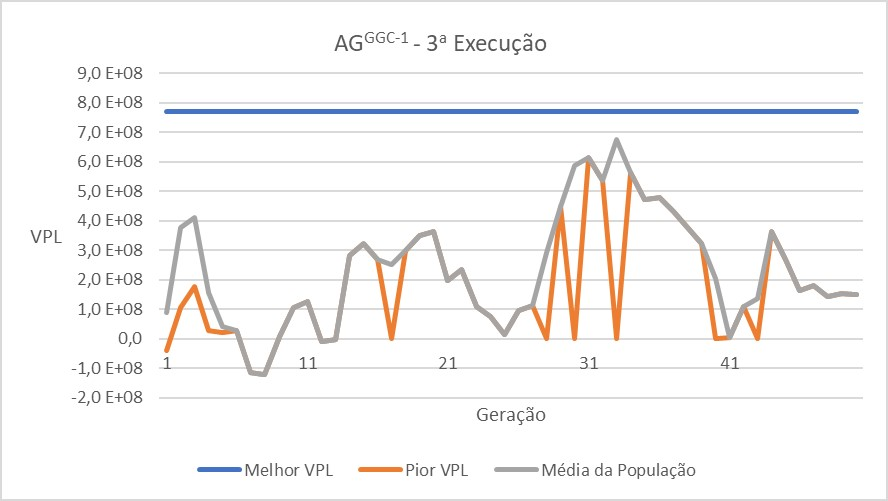
\includegraphics[scale=1]{ApA/GCC/3}
\end{figure}

\begin{figure}[H]
\centering

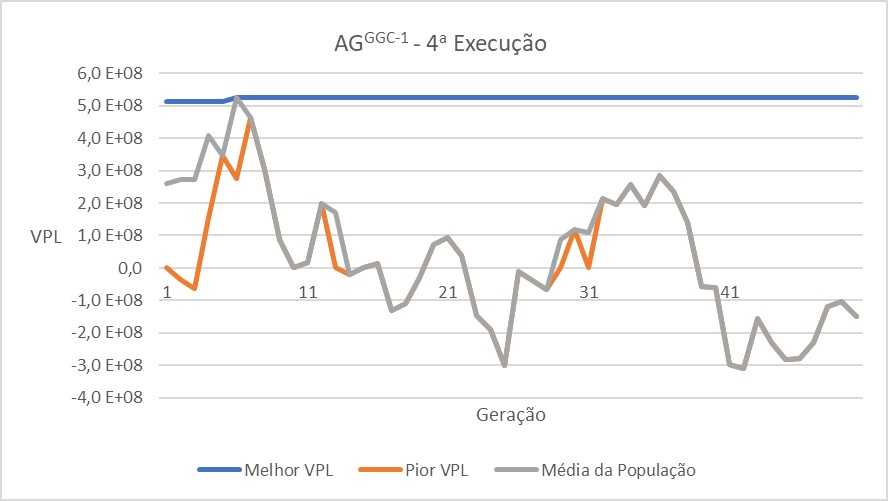
\includegraphics[scale=1]{ApA/GCC/4}
\end{figure}

\begin{figure}[htb]
\centering

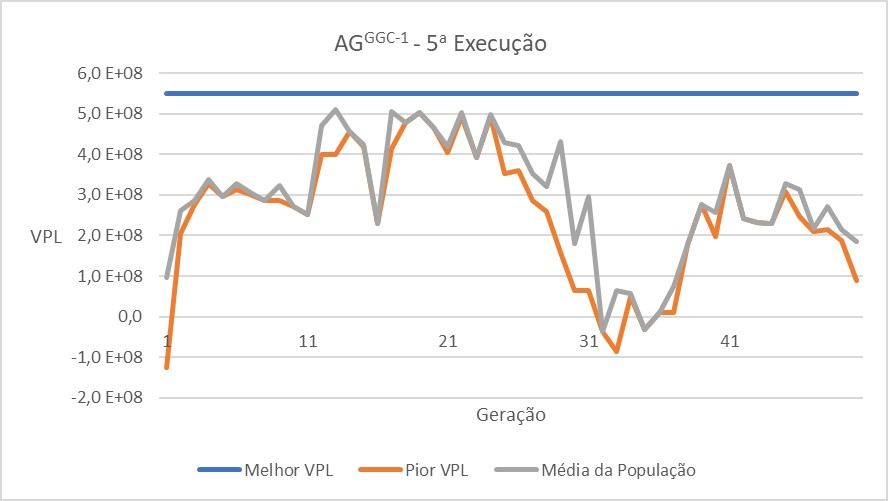
\includegraphics[scale=1]{ApA/GCC/5}
\end{figure}


\begin{figure}[H]
\centering

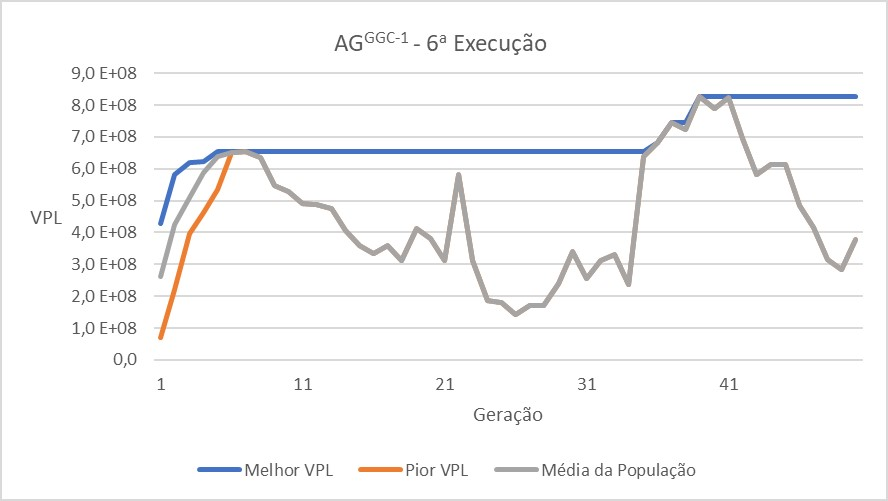
\includegraphics[scale=1]{ApA/GCC/6}
\end{figure}

\begin{figure}[H]
\centering

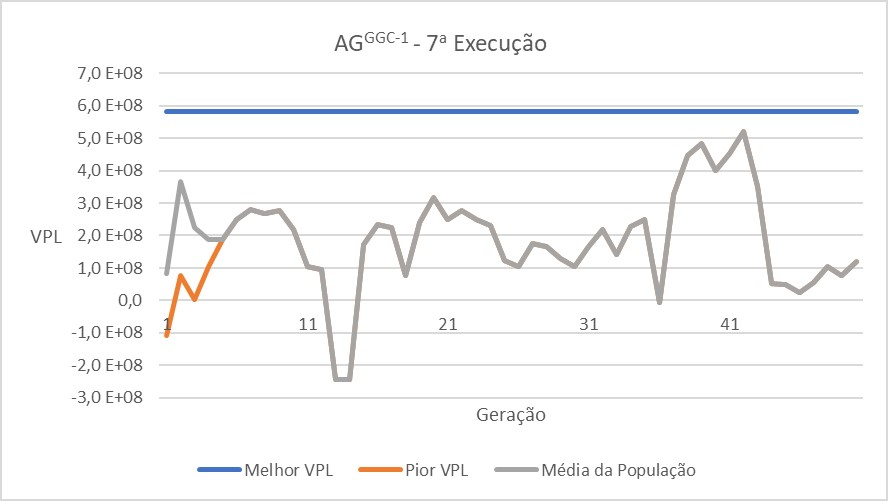
\includegraphics[scale=1]{ApA/GCC/7}
\end{figure}

\begin{figure}[H]
\centering

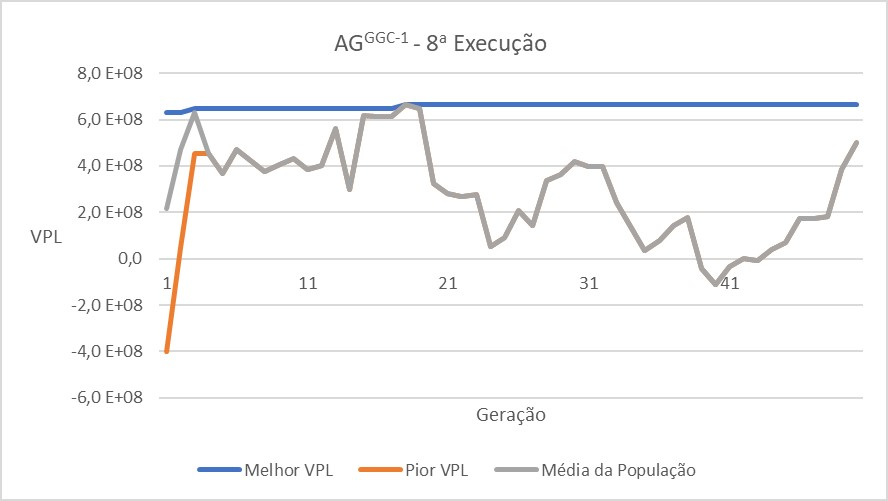
\includegraphics[scale=1]{ApA/GCC/8}
\end{figure}

\begin{figure}[H]
\centering

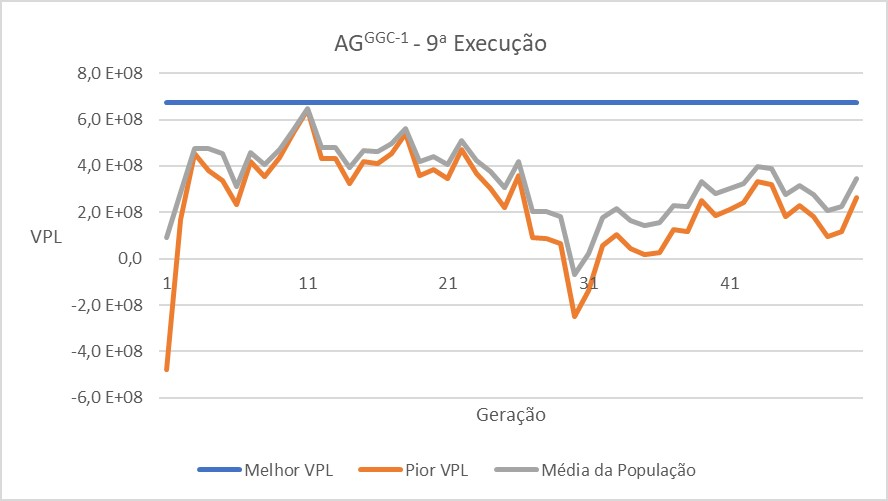
\includegraphics[scale=1]{ApA/GCC/9}
\end{figure}

\begin{figure}[H]
\centering

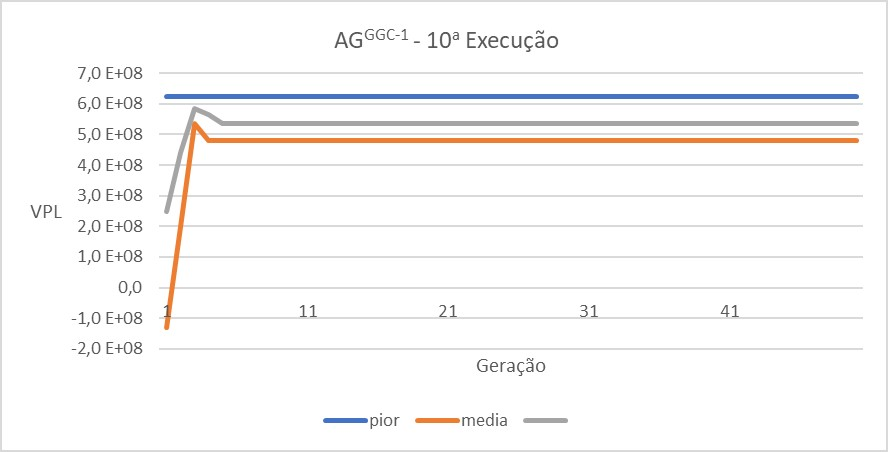
\includegraphics[scale=1]{ApA/GCC/10}
\end{figure}

\subsubsection{AGRPC}

\begin{figure}[H]
\centering

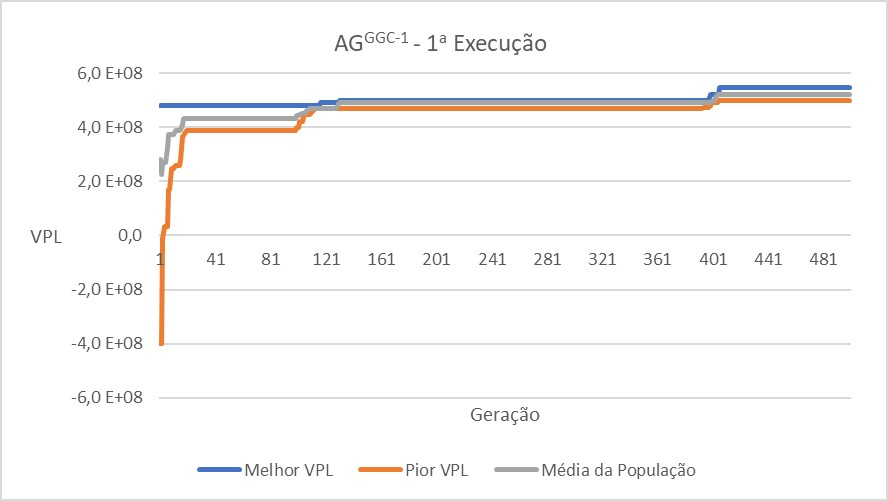
\includegraphics[scale=1]{ApA/AGRPC/1}
\end{figure}

\begin{figure}[H]
\centering

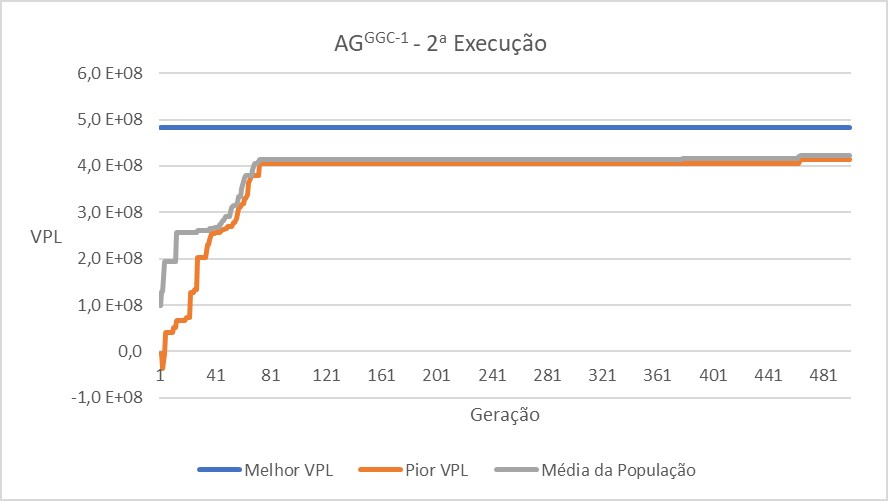
\includegraphics[scale=1]{ApA/AGRPC/2}
\end{figure}

\begin{figure}[H]
\centering

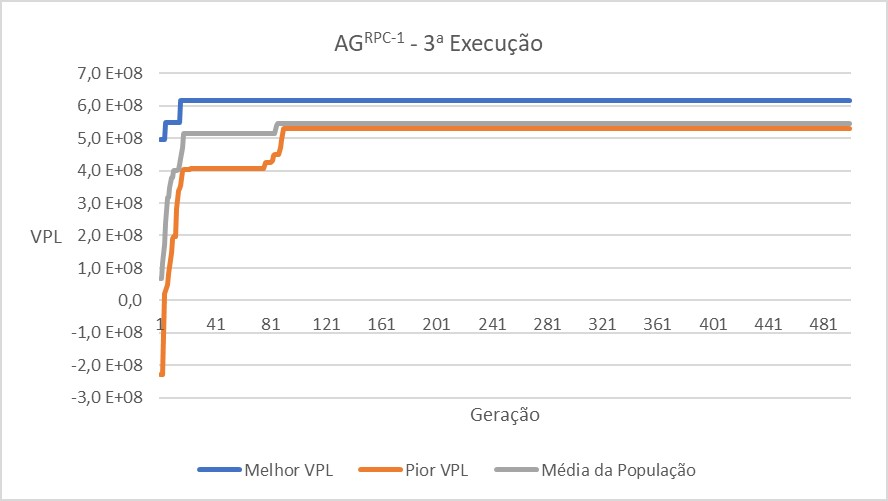
\includegraphics[scale=1]{ApA/AGRPC/3}
\end{figure}

\begin{figure}[H]
\centering

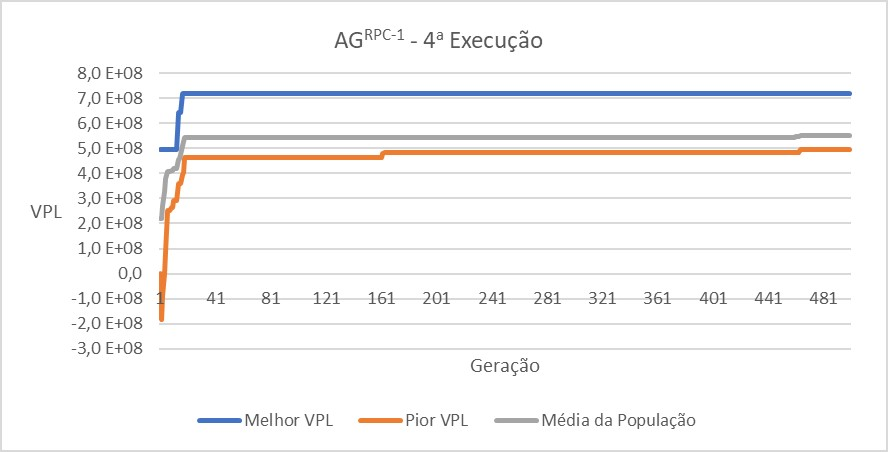
\includegraphics[scale=1]{ApA/AGRPC/4}
\end{figure}

\begin{figure}[H]
\centering

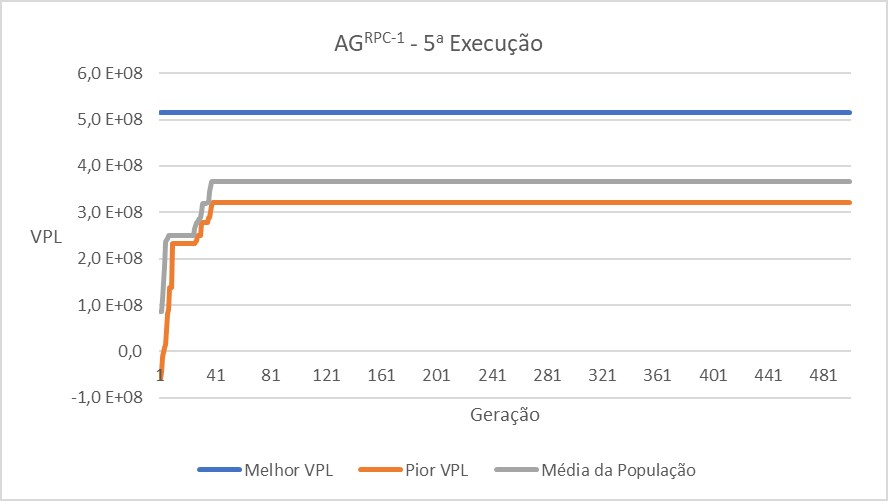
\includegraphics[scale=1]{ApA/AGRPC/5}
\end{figure}

\begin{figure}[H]
\centering

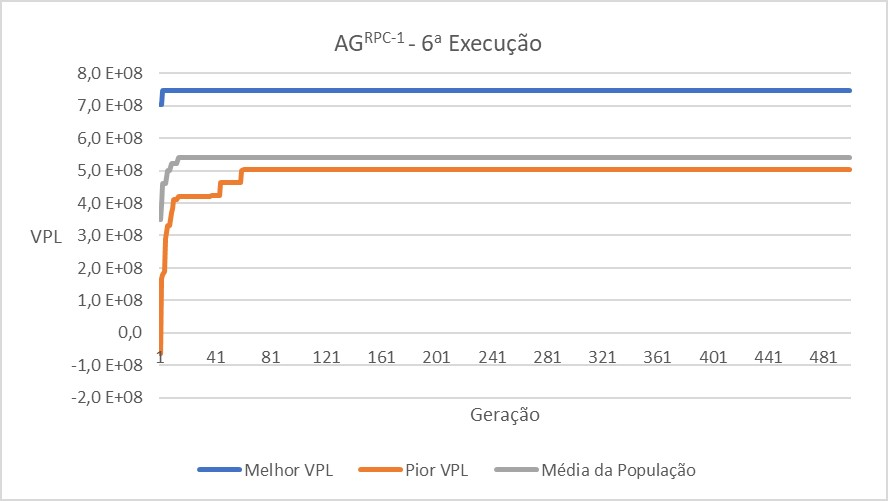
\includegraphics[scale=1]{ApA/AGRPC/6}
\end{figure}

\begin{figure}[H]
\centering

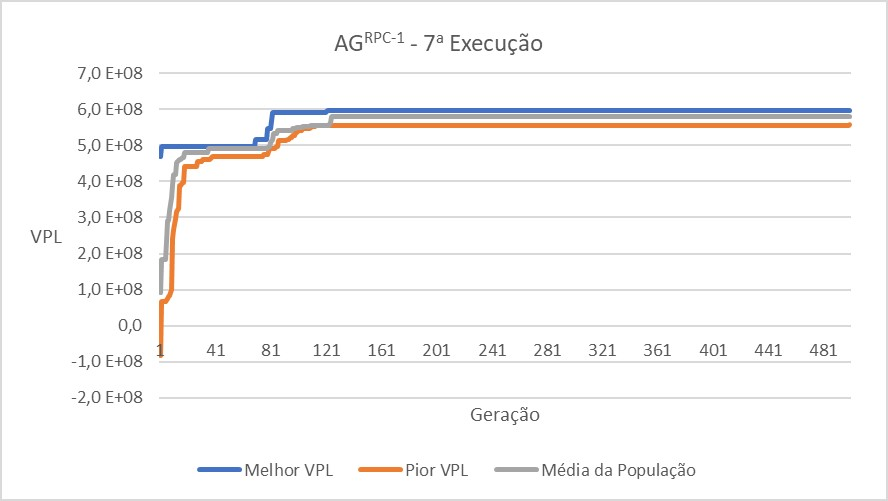
\includegraphics[scale=1]{ApA/AGRPC/7}
\end{figure}

\begin{figure}[H]
\centering

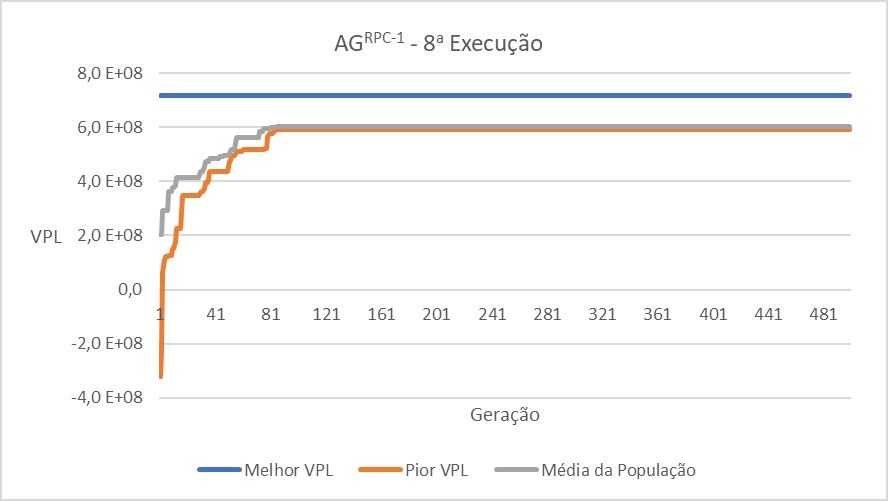
\includegraphics[scale=1]{ApA/AGRPC/8}
\end{figure}

\begin{figure}[H]
\centering

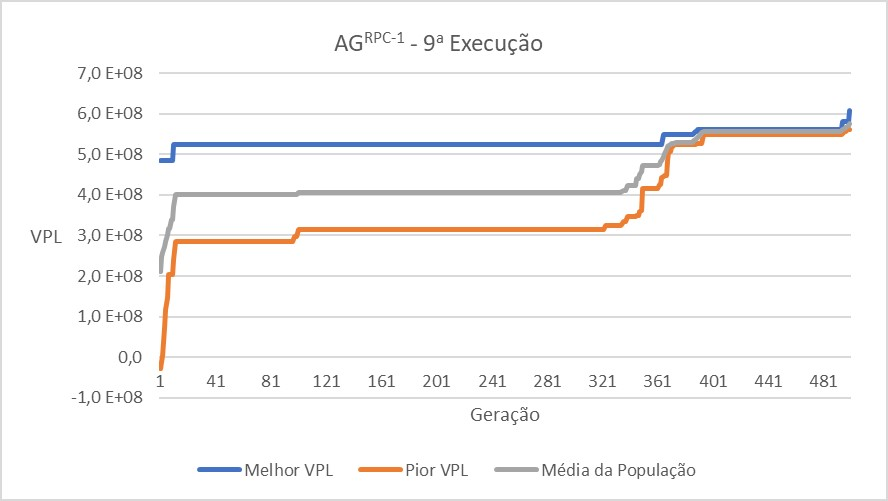
\includegraphics[scale=1]{ApA/AGRPC/9}
\end{figure}

\begin{figure}[H]
\centering

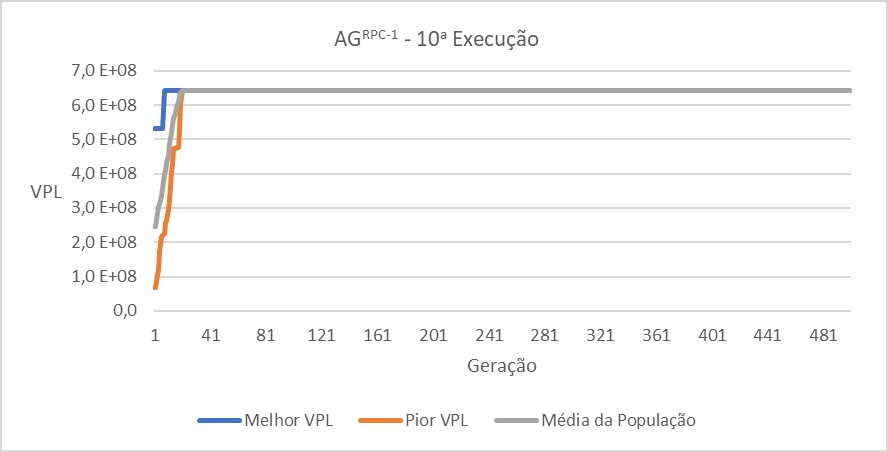
\includegraphics[scale=1]{ApA/AGRPC/10}
\end{figure}

\chapter{}
\subsubsection{Algoritmo Genético Geracional}

\begin{figure}[H]
\centering

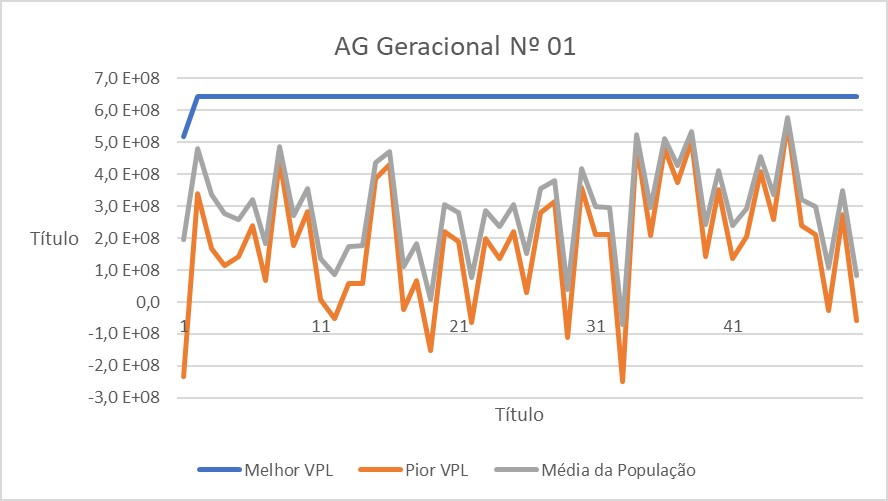
\includegraphics[scale=1]{ApB/AGG/1}

\end{figure}

\begin{figure}[H]
\centering

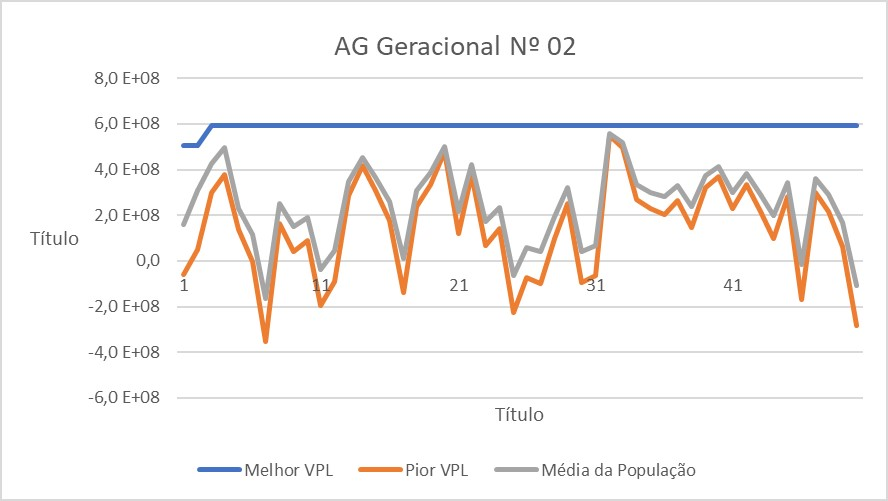
\includegraphics[scale=1]{ApB/AGG/2}

\end{figure}

\begin{figure}[H]
\centering

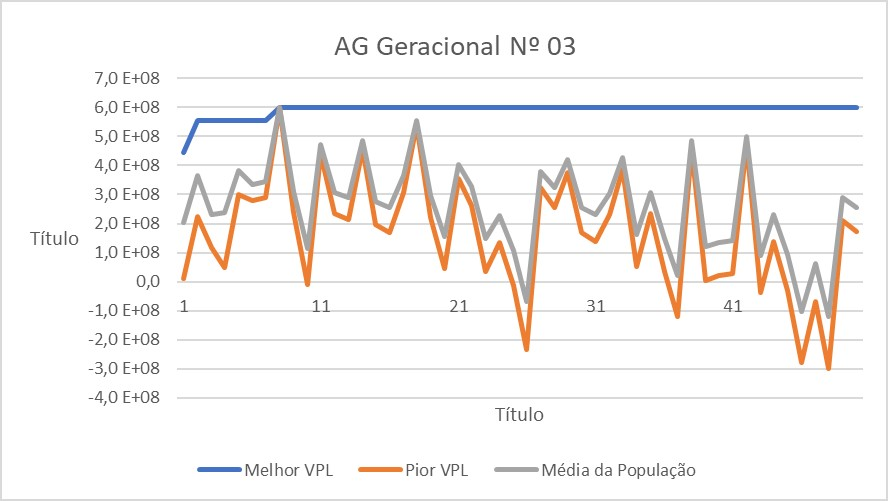
\includegraphics[scale=1]{ApB/AGG/3}

\end{figure}

\begin{figure}[H]
\centering

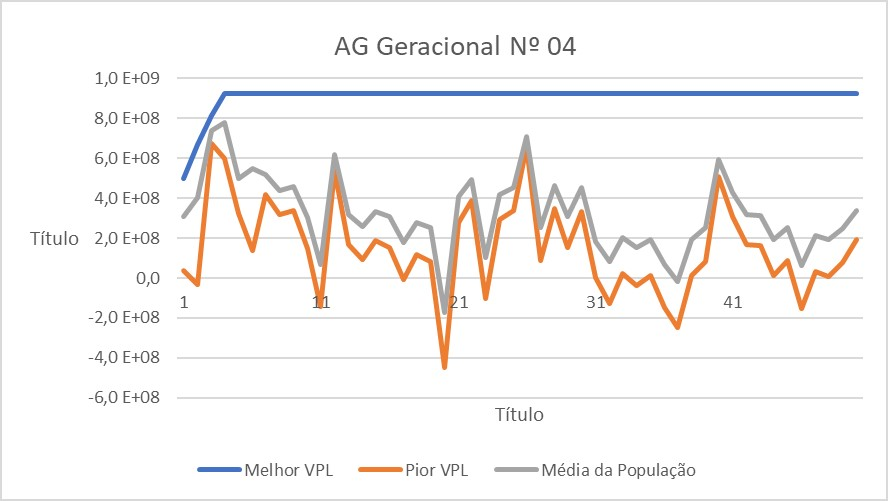
\includegraphics[scale=1]{ApB/AGG/4}

\end{figure}

\begin{figure}[H]
\centering

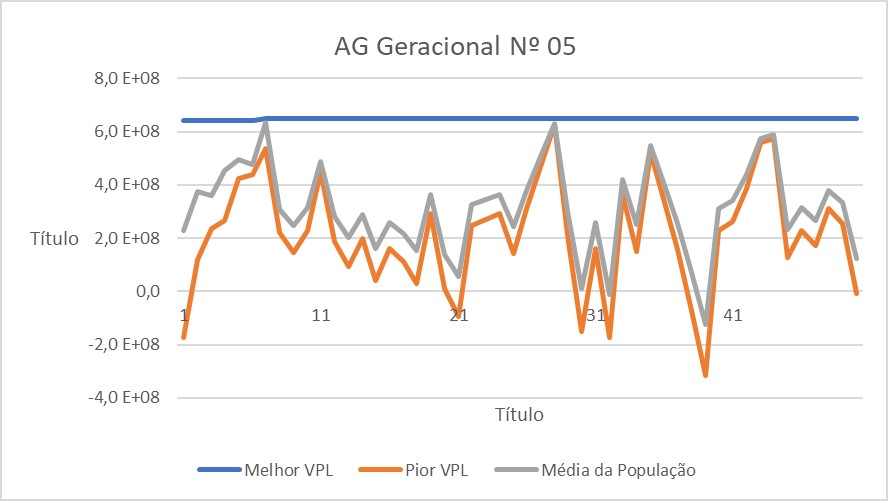
\includegraphics[scale=1]{ApB/AGG/5}

\end{figure}

\begin{figure}[H]
\centering

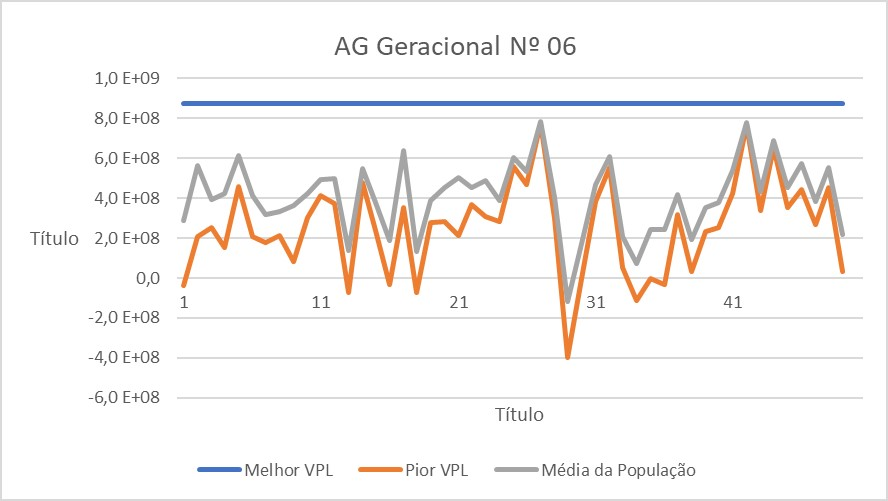
\includegraphics[scale=1]{ApB/AGG/6}

\end{figure}

\begin{figure}[H]
\centering

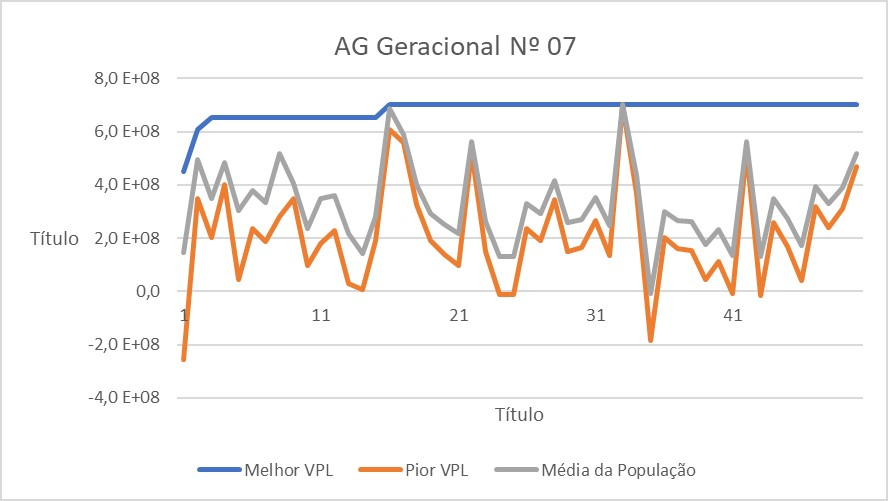
\includegraphics[scale=1]{ApB/AGG/7}

\end{figure}

\begin{figure}[H]
\centering

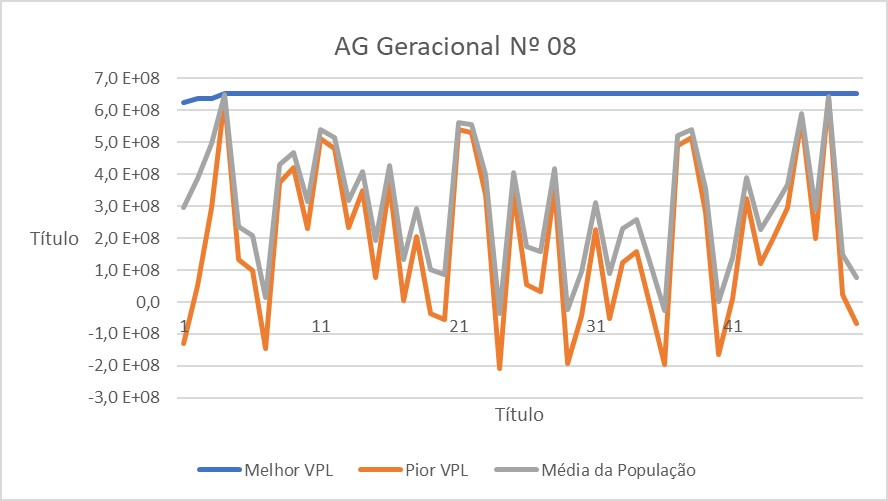
\includegraphics[scale=1]{ApB/AGG/8}

\end{figure}

\begin{figure}[H]
\centering

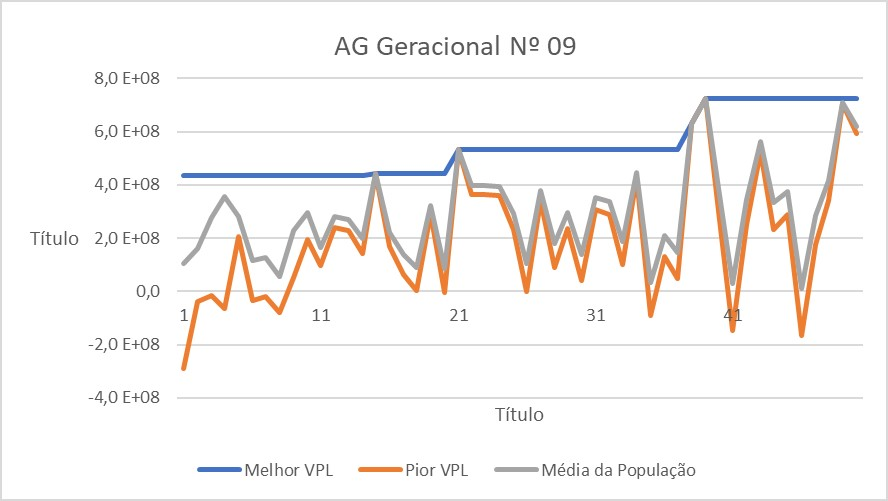
\includegraphics[scale=1]{ApB/AGG/9}

\end{figure}

\begin{figure}[H]
\centering

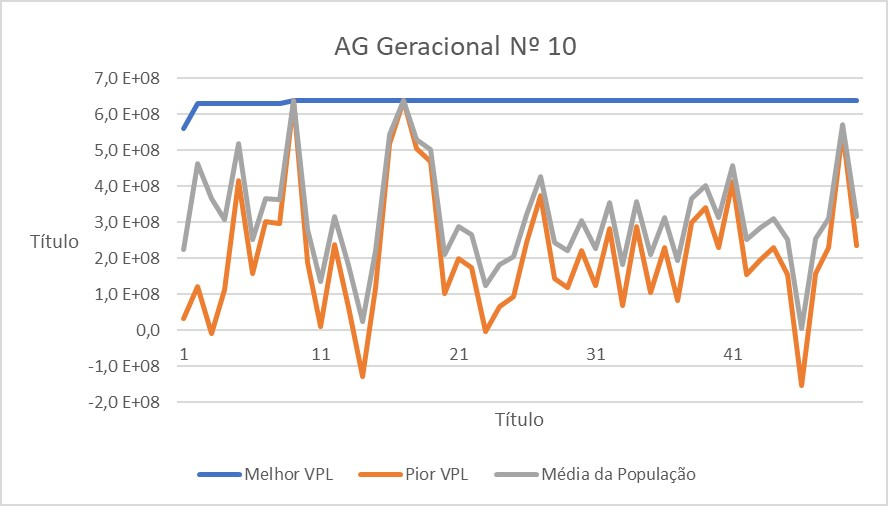
\includegraphics[scale=1]{ApB/AGG/10}

\end{figure}

\subsubsection{Algoritmo Genético de Regime Permanente}

\begin{figure}[H]
\centering

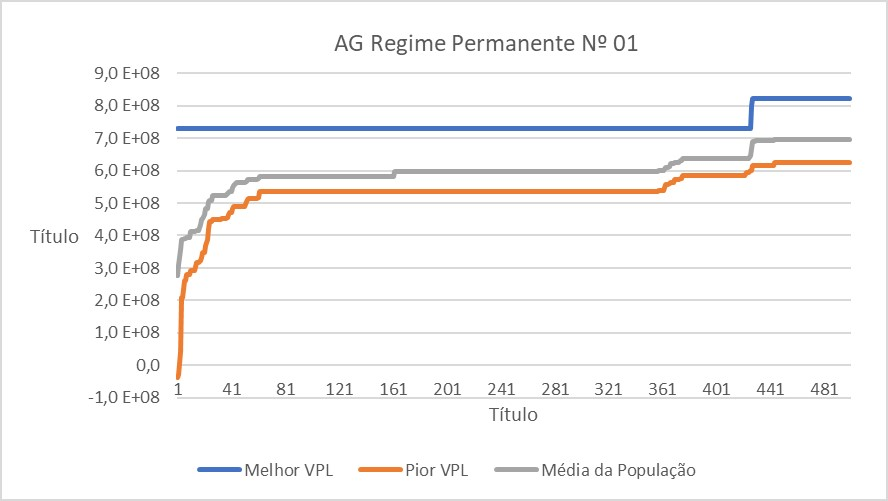
\includegraphics[scale=1]{ApB/AGRP/1}

\end{figure}

\begin{figure}[H]
\centering

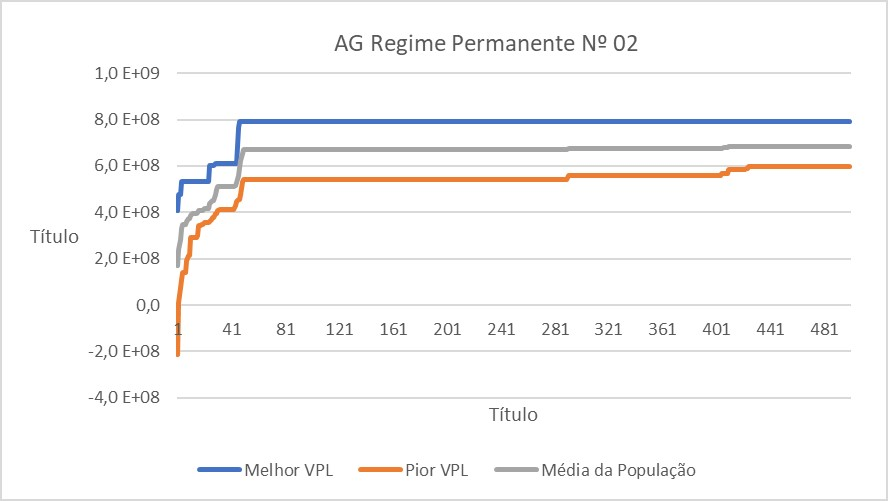
\includegraphics[scale=1]{ApB/AGRP/2}

\end{figure}

\begin{figure}[H]
\centering

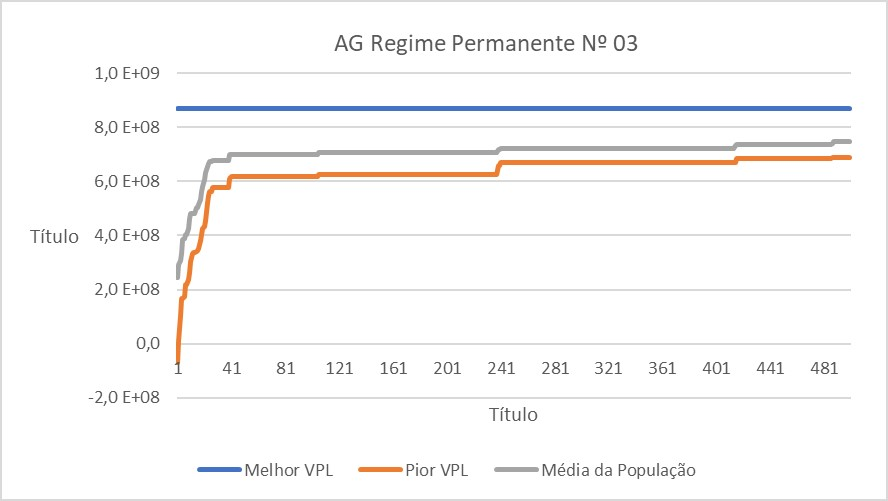
\includegraphics[scale=1]{ApB/AGRP/3}

\end{figure}

\begin{figure}[H]
\centering

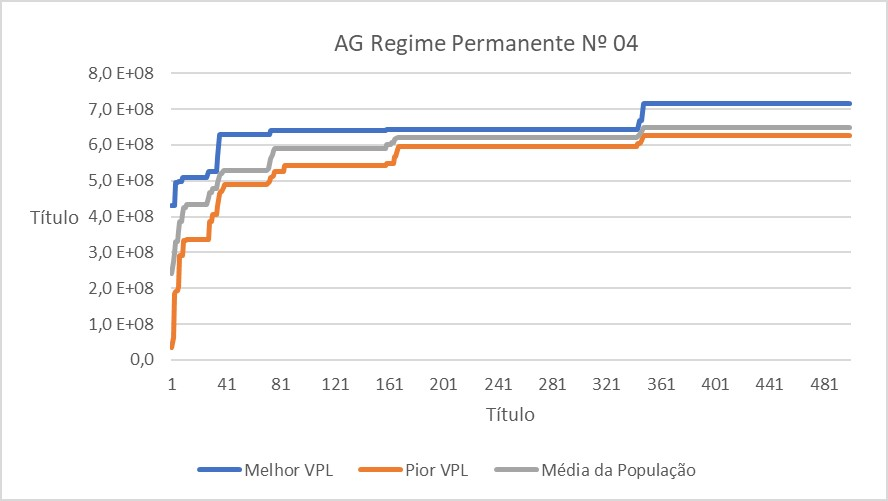
\includegraphics[scale=1]{ApB/AGRP/4}

\end{figure}

\begin{figure}[H]
\centering

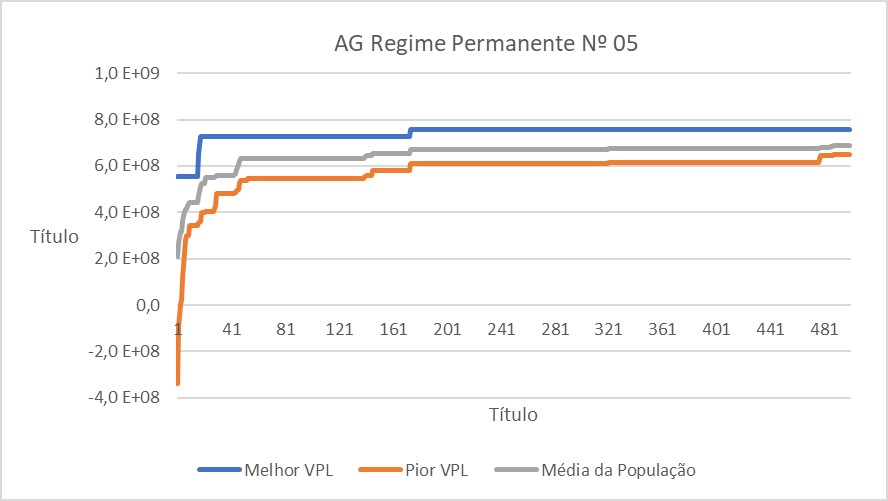
\includegraphics[scale=1]{ApB/AGRP/5}

\end{figure}

\begin{figure}[H]
\centering

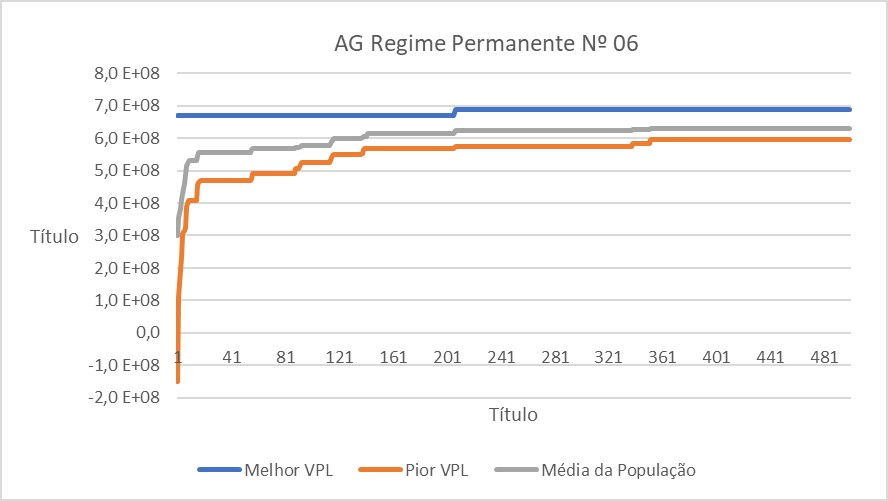
\includegraphics[scale=1]{ApB/AGRP/6}

\end{figure}

\begin{figure}[H]
\centering

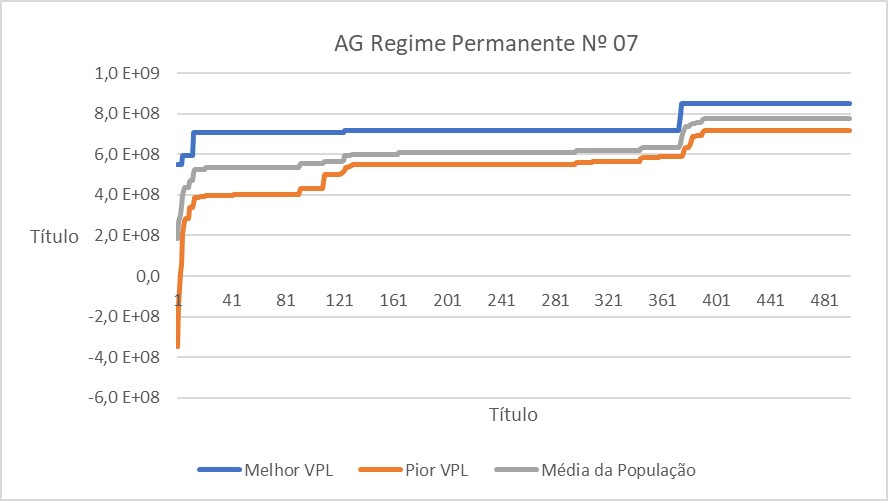
\includegraphics[scale=1]{ApB/AGRP/7}

\end{figure}

\begin{figure}[H]
\centering

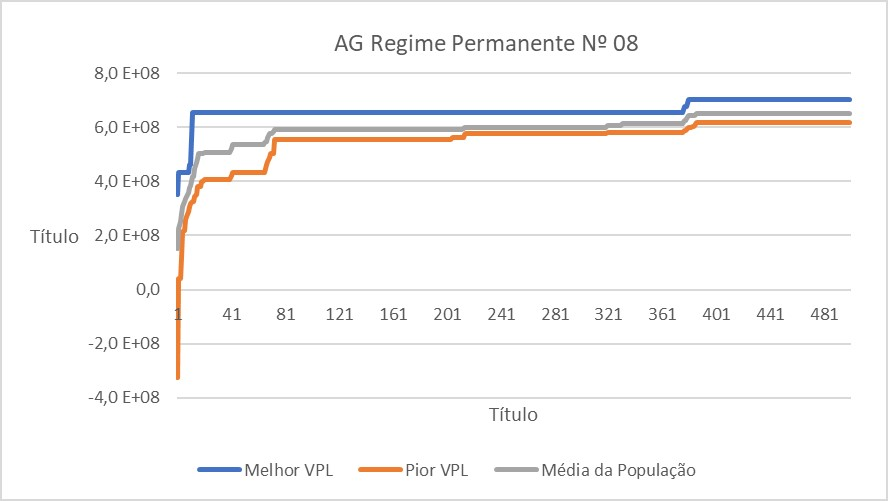
\includegraphics[scale=1]{ApB/AGRP/8}

\end{figure}


\begin{figure}[H]
\centering

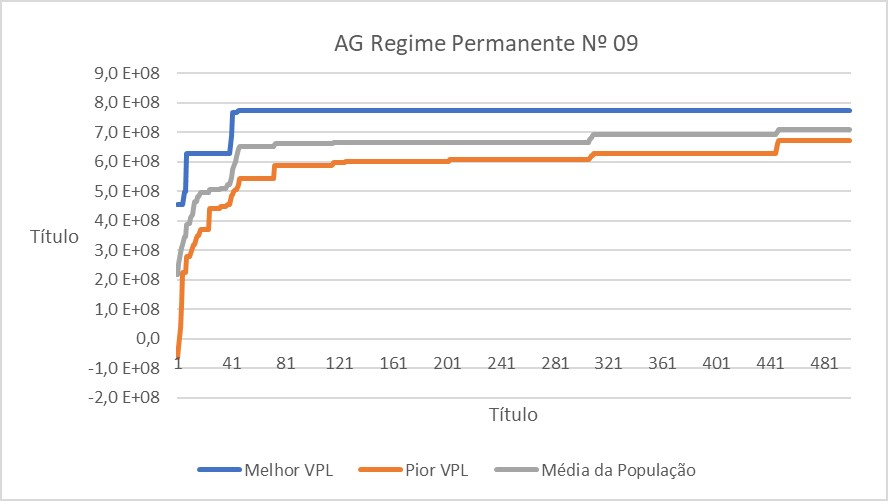
\includegraphics[scale=1]{ApB/AGRP/9}

\end{figure}

\begin{figure}[H]
\centering

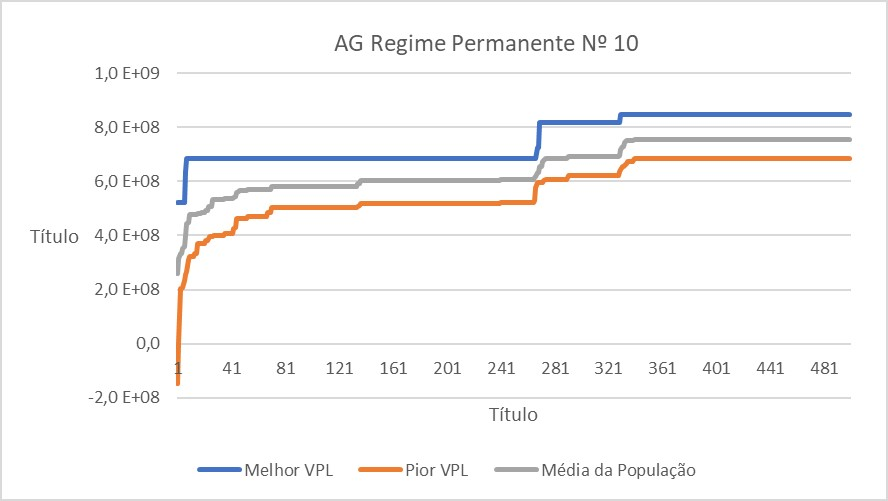
\includegraphics[scale=1]{ApB/AGRP/10}

\end{figure}

\chapter{}
\subsubsection{Algoritmo Genético Geracional}

\begin{figure}[H]
\centering

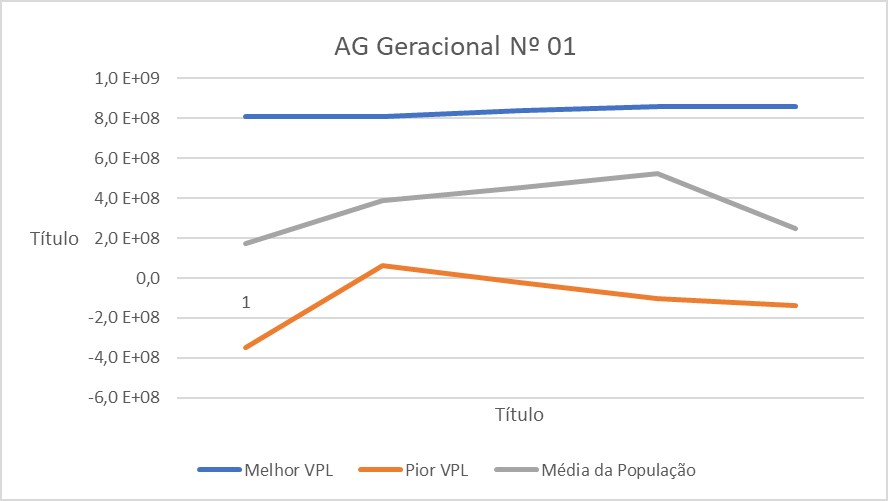
\includegraphics[scale=1]{ApC/AGG/1}

\end{figure}

\begin{figure}[H]
\centering

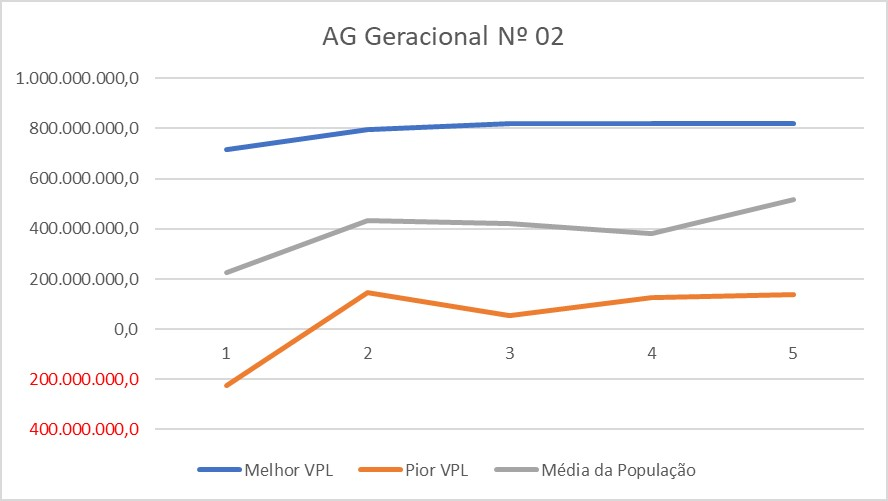
\includegraphics[scale=1]{ApC/AGG/2}

\end{figure}

\begin{figure}[H]
\centering

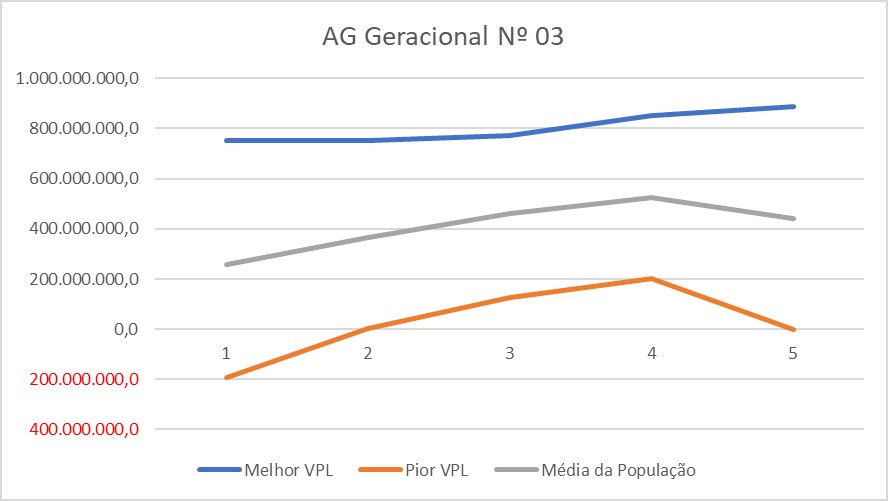
\includegraphics[scale=1]{ApC/AGG/3}

\end{figure}

\begin{figure}[H]
\centering

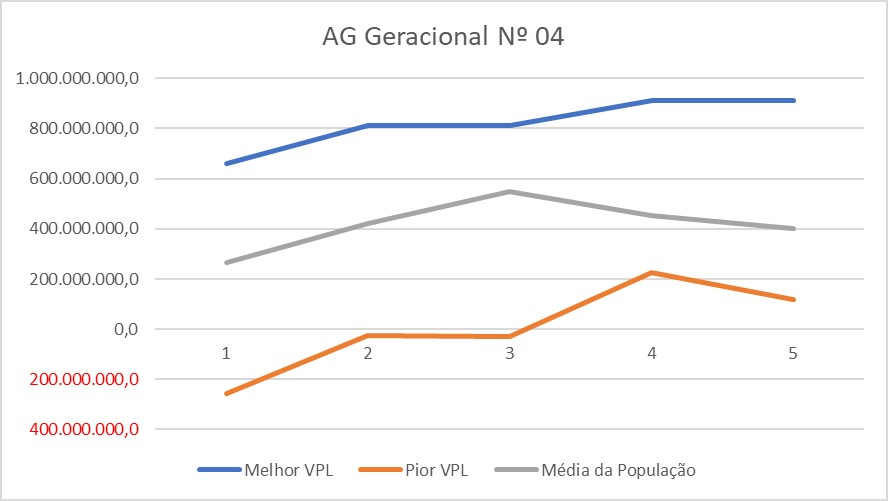
\includegraphics[scale=1]{ApC/AGG/4}

\end{figure}

\begin{figure}[H]
\centering

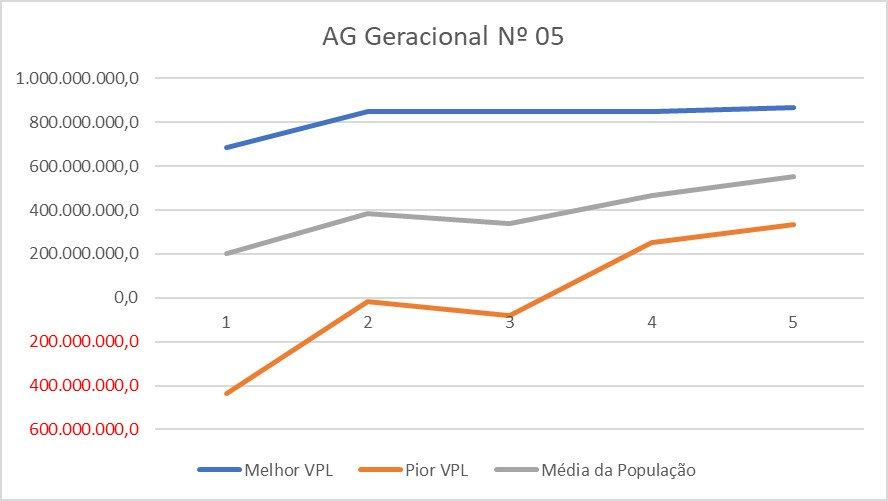
\includegraphics[scale=1]{ApC/AGG/5}

\end{figure}

\begin{figure}[H]
\centering

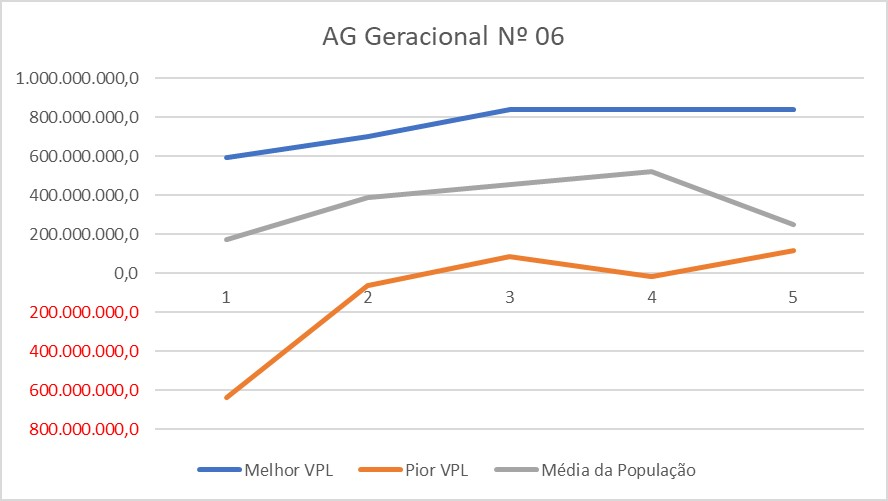
\includegraphics[scale=1]{ApC/AGG/6}

\end{figure}

\begin{figure}[H]
\centering

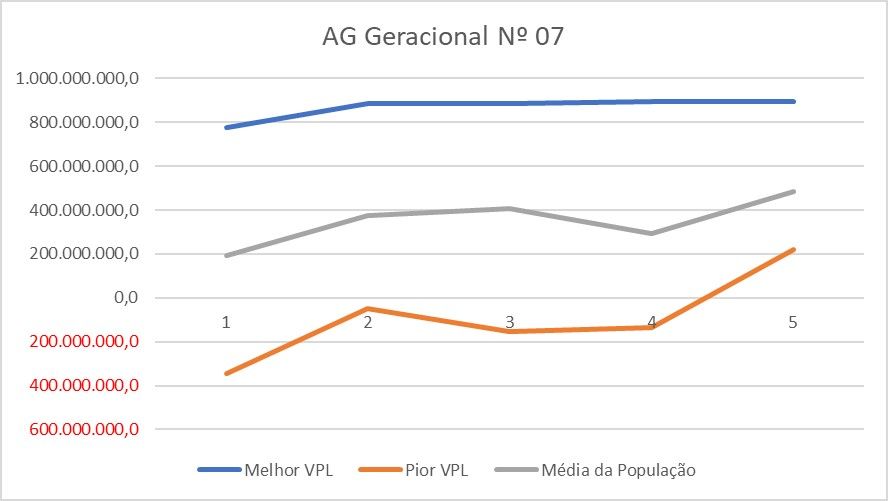
\includegraphics[scale=1]{ApC/AGG/7}

\end{figure}

\begin{figure}[H]
\centering

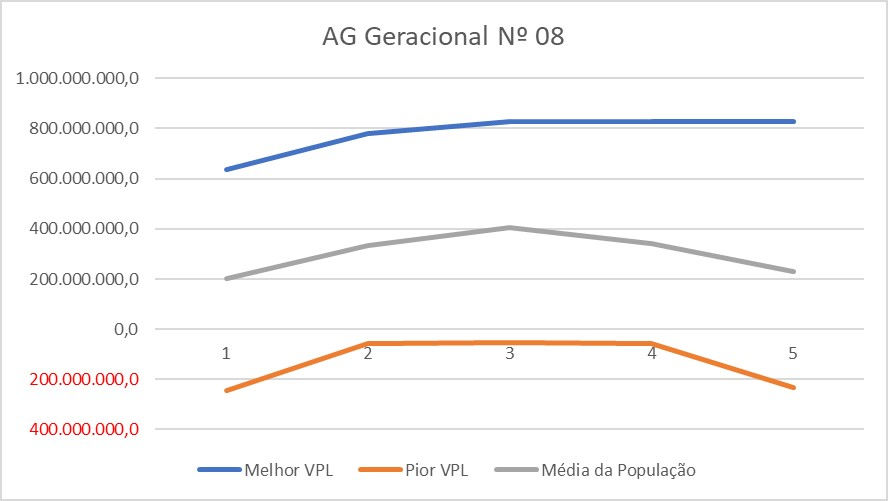
\includegraphics[scale=1]{ApC/AGG/8}

\end{figure}

\begin{figure}[H]
\centering

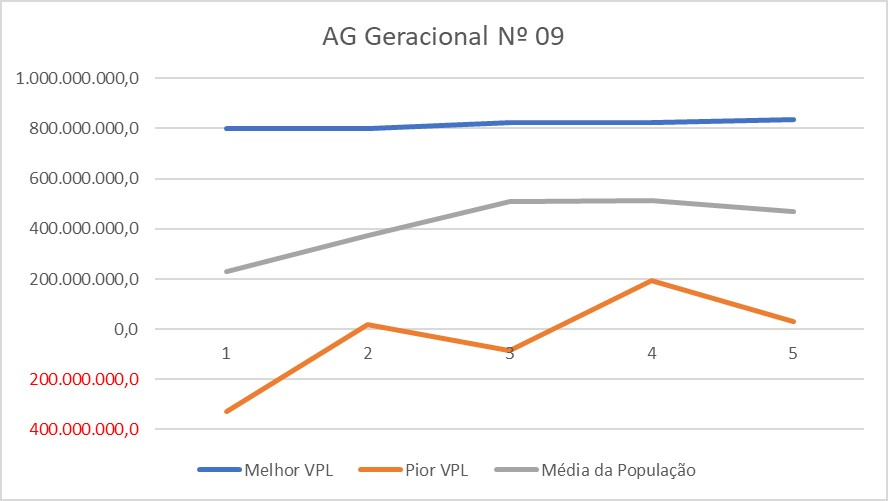
\includegraphics[scale=1]{ApC/AGG/9}

\end{figure}

\begin{figure}[H]
\centering

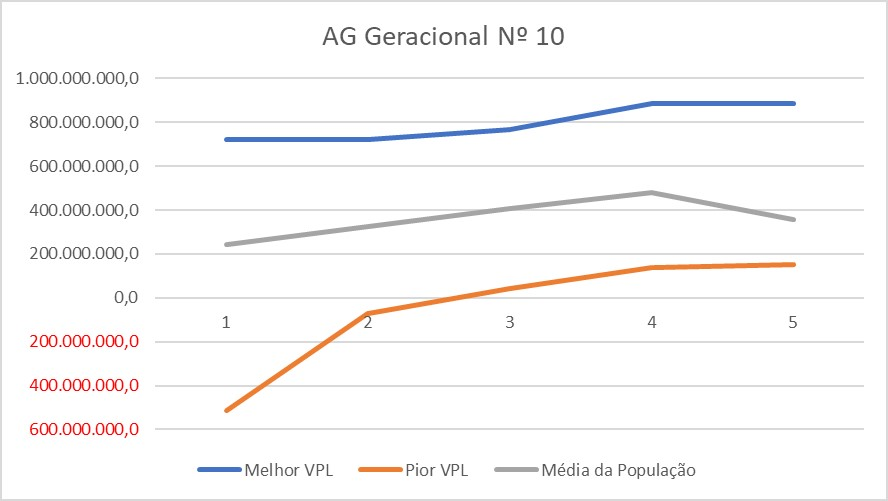
\includegraphics[scale=1]{ApC/AGG/10}

\end{figure}

\subsubsection{Algoritmo Genético de Regime Permanente} 

\begin{figure}[H]
\centering

\includegraphics[scale=1]{ApC/AGRP/1}

\end{figure}

\begin{figure}[H]
\centering

\includegraphics[scale=1]{ApC/AGRP/2}

\end{figure}
\begin{figure}[H]
\centering

\includegraphics[scale=1]{ApC/AGRP/3}

\end{figure}
\begin{figure}[H]
\centering

\includegraphics[scale=1]{ApC/AGRP/4}

\end{figure}
\begin{figure}[H]
\centering

\includegraphics[scale=1]{ApC/AGRP/5}

\end{figure}
\begin{figure}[H]
\centering

\includegraphics[scale=1]{ApC/AGRP/6}

\end{figure}
\begin{figure}[H]
\centering

\includegraphics[scale=1]{ApC/AGRP/7}

\end{figure}
\begin{figure}[H]
\centering

\includegraphics[scale=1]{ApC/AGRP/8}

\end{figure}
\begin{figure}[H]
\centering

\includegraphics[scale=1]{ApC/AGRP/9}

\end{figure}
\begin{figure}[H]
\centering

\includegraphics[scale=1]{ApC/AGRP/10}

\end{figure}

\chapter{}
\subsubsection{Algoritmo Genético de Regime Permanente Modificado}

\begin{figure}[H]
\centering

\includegraphics[scale=1]{ApD/1}

\end{figure}

\begin{figure}[H]
\centering

\includegraphics[scale=1]{ApD/2}

\end{figure}


\begin{figure}[H]
\centering

\includegraphics[scale=1]{ApD/3}

\end{figure}

\begin{figure}[H]
\centering

\includegraphics[scale=1]{ApD/4}

\end{figure}


\begin{figure}[H]
\centering

\includegraphics[scale=1]{ApD/5}

\end{figure}

\begin{figure}[H]
\centering

\includegraphics[scale=1]{ApD/6}

\end{figure}

\begin{figure}[H]
\centering

\includegraphics[scale=1]{ApD/7}

\end{figure}

\begin{figure}[H]
\centering

\includegraphics[scale=1]{ApD/8}

\end{figure}

\begin{figure}[H]
\centering

\includegraphics[scale=1]{ApD/9}

\end{figure}

\begin{figure}[H]
\centering

\includegraphics[scale=1]{ApD/10}

\end{figure}

\chapter{}
\subsubsection{Algoritmo Genético de Regime Permanente com Contador de Ocorrências 1ª Versão}


\begin{figure}[H]
\centering

\includegraphics[scale=1]{ApE/AGRPCO1/1}

\end{figure}

\begin{figure}[H]
\centering

\includegraphics[scale=1]{ApE/AGRPCO1/2}

\end{figure}

\begin{figure}[H]
\centering

\includegraphics[scale=1]{ApE/AGRPCO1/3}

\end{figure}
\begin{figure}[H]
\centering

\includegraphics[scale=1]{ApE/AGRPCO1/4}

\end{figure}
\begin{figure}[H]
\centering

\includegraphics[scale=1]{ApE/AGRPCO1/5}

\end{figure}
\begin{figure}[H]
\centering

\includegraphics[scale=1]{ApE/AGRPCO1/6}

\end{figure}
\begin{figure}[H]
\centering

\includegraphics[scale=1]{ApE/AGRPCO1/7}

\end{figure}
\begin{figure}[H]
\centering

\includegraphics[scale=1]{ApE/AGRPCO1/8}

\end{figure}
\begin{figure}[H]
\centering

\includegraphics[scale=1]{ApE/AGRPCO1/9}

\end{figure}
\begin{figure}[H]
\centering

\includegraphics[scale=1]{ApE/AGRPCO1/10}

\end{figure}

\subsubsection{Algoritmo Genético de Regime Permanente com Contador de Ocorrências 2ª Versão}


\begin{figure}[H]
\centering

\includegraphics[scale=1]{ApE/AGRPCO2/1}

\end{figure}

\begin{figure}[H]
\centering

\includegraphics[scale=1]{ApE/AGRPCO2/2}

\end{figure}

\begin{figure}[H]
\centering

\includegraphics[scale=1]{ApE/AGRPCO2/3}

\end{figure}

\begin{figure}[H]
\centering

\includegraphics[scale=1]{ApE/AGRPCO2/4}

\end{figure}

\begin{figure}[H]
\centering

\includegraphics[scale=1]{ApE/AGRPCO2/5}

\end{figure}

\begin{figure}[H]
\centering

\includegraphics[scale=1]{ApE/AGRPCO2/6}

\end{figure}

\begin{figure}[H]
\centering

\includegraphics[scale=1]{ApE/AGRPCO2/7}

\end{figure}

\begin{figure}[H]
\centering

\includegraphics[scale=1]{ApE/AGRPCO2/8}

\end{figure}

\begin{figure}[H]
\centering

\includegraphics[scale=1]{ApE/AGRPCO2/9}

\end{figure}

\begin{figure}[H]
\centering

\includegraphics[scale=1]{ApE/AGRPCO2/10}

\end{figure}
\end{document}